\documentclass[10pt]{article}
\usepackage[utf8]{inputenc}
\usepackage[MeX]{polski}
\usepackage{graphicx}
\usepackage{amsmath,amssymb,amsfonts}
\usepackage{pdfpages} % paczka żeby móc importować gotowe strony z plików pdf do pdfa z latexa
\usepackage{titlesec} % może być potrzebne jeśli będziemy chcieli edytować tytuły
\usepackage{tocloft}  % żeby móc ręcznie dodawać sections do TOC (Table of Content)
\usepackage[nottoc]{tocbibind}  % definiuje co jest w TOC
% nottoc -  Disables the inclusion of the ToC.

% to powyższe można zastąpić 2 liniami:
% \usepackage{tocbibind}
% \tocbibind{nottoc}

\usepackage{geometry} % Do ustawiania wyglądu stron
\geometry{margin=1.2in} % Ustawia margines

\usepackage{sectsty}  % Chyba żeby móc ustawić baselineskip i linespread
\usepackage{indentfirst}  % Ustawienia aby pierwszy paragraf w sekcji też miał akapit, bo domyślnie nie ma

\usepackage{graphicx} % Do załączania obrazów
\graphicspath{ {./images/} }

\usepackage{chngcntr} % Do edycji numerowania rysunków w sekcjach
\counterwithin{figure}{section} % Sprawia, że numeracja rysunków będzie podzielona na sekcje

\usepackage{csquotes} % Do cytowania
\AtBeginEnvironment{quote}{\itshape}  % Ustawia to co jest między \begin{quote}
% a \end{quote}, że będzie kursywą

%\renewcommand{\chaptername}{Rozdział}
%\renewcommand{\contentsname}{Spis treści}
%\renewcommand{\figurename}{Rys.}
%\renewcommand{\tablename}{Tab.}
%\renewcommand{\listfigurename}{Spis rysunków}
%\renewcommand{\listtablename}{Spis tabel}
%\renewcommand{\bibname}{Bibliografia}

% Chyba lepiej używać latexowego \indent zamiast definiować własny akapit
% \newcommand\tab[1][1cm]{\hspace*{#1}}
% \newcommand\tab{\indent}

\pagestyle{plain}
\pagenumbering{arabic}
\sectionfont{\fontsize{13}{15}\selectfont}  % Ustawia wielkośc czcionki tytułów sekcji
% First {} is a font size for title of sections and second {} is baselineskip,
% that is size of empty space between section title and text below

\widowpenalties 1 10000
\raggedbottom

\begin{document}

\parskip 1.5ex % paragraph spacing - zwiększa odstępy pomiędzy paragrafami

\baselineskip=15pt  % odległość między liniami chyba
\linespread{1.3} % W wymogach jest, że ma być  1.5, ale podobno ten końcowy line spacing
% wylicza się jako ten linespread * (baselineskip/fontsize) i w naszym przypadku
% to powinno być 1.25 * (12/10) = 1.5, no ale zobaczymy bo aktualnie ten parametr wygląda jakby nie działał

% Strone tytulowa trzeba bedzie pobrac z moja pg

\includepdf[pages=-]{StronaTytulowa_bb.pdf} %pages=- to załączenie wszystkich stron


\begin{titlepage}
  \begin{center}

    \vspace*{1cm}
    \Huge
    \textbf{POLITECHNIKA GDAŃSKA}
    \newline
    \vspace{0.5cm}
    \LARGE
    Katedra Systemów Decyzyjnych i Robotyki

    \vspace{1.5cm}
    \textbf{PRACA INŻYNIERSKA}
    \\[0.5cm]
    \textbf{Zastosowanie sieci neuronowych do edycji obrazów}

    \vspace{2.5cm}
    \Large
    \textbf{Autorzy}\\
    Piotr Winkler\\
    Bartosz Bieliński

    \vspace{3.5cm}
    Gdańsk 2019

  \end{center}
\end{titlepage}

\setcounter{page}{2}

\section*{Streszczenie}

  Tematem pracy jest zbadanie możliwości zastosowania sieci neuronowych do
  edycji obrazów. Głównym celem było stworzenie narzędzi opartych na wyuczonych
  sieciach neuronowych, służących do odpowiedniego przetwarzania i
  modyfikowania obrazu. Następnie skuteczność tych narzędzi została oceniona i
  porównana z rozwiązaniami opartymi na klasycznych metodach przetwarzania obrazu.

  Zbadane zostały dwie problematyki, automatyczne kolorowanie czarno-białych obrazów
  oraz nakładanie na obraz prostych filtrów takich jak wykrywający
  krawędzie filtr Sobela-Feldmana. Opisy zaimplementowanych rozwiązań zostały
  umieszczone w odpowiednych podrozdziałach
  rozdziału \ref{zaimplementowane rozwiazania}.

  Uzyskane wyniki pozwoliły dojść do wielu konstruktywnych obserwacji. W przypadku obu
  problematyk udało się je rozwiązać z użyciem rozwiązań opartych na konwolucyjnych
  sieciach neuronowych.

  W celu ułatwienia przeprowadzania badań została opracowana specjalna platforma
  programistyczna o nazwie \textit{TorchFrame}. Ma on za zadanie kontrolować
  przepływ danych w procesie uczenia i testowania badanych modeli, a co za tym
  idzie, ograniczyć konieczność ingerencji ze strony użytkownika. Przekłada
  się to na znacznie wydajniejszy oraz mniej złożony proces trenowania
  różnorodnych architektur sieci neuronowych.

  W przypadku prostych filtrów obrazu rozwiązania
  oparte na sieciach splotowych okazały się wolniejsze i bardziej pracochłonne w
  implementacji niż metody klasyczne przy porównywalnych rezultatach. Jednakże
  z ich pomocą udało się udowodnić olbrzymią uniwersalność sieci splotowych
  mogących być efektywnie zastosowane w zagadnieniach związanych z prostym
  przetwarzaniem obrazu.

  Zagadnienie automatycznego kolorowania czarno-białych
  obrazów zostało rozwiązane z użyciem dwóch różnych modeli, autorskiego modelu
  prostego oraz bardziej zaawansowanego modelu zaimplementowanego z użyciem technik
  przeniesienia uczenia. Dla modelu autorskiego zostały przeprowadzone szczegółowe
  badania dotyczące zależności wyników od poszczególnych parametrów architekury
  sieci jak i konfiguracji procesu uczenia. Rezultaty końcowe uzyskane z użyciem
  modelu autorskiego były zadowalające, ale mocno zależne od wybranych parametrów.
  Dowodzi to, że odpowiednio skonfigurowane sieci splotowe mogą być skutecznie
  zastosowane w tym zagadnieniu, aczkolwiek to model złożony pozwolił osiągnąć
  największy sukces.
  Idea tego rozwiązania opiera się na integracji cech obrazu średniego oraz wysokiego
  poziomu uzyskiwanych z użyciem złożonej sieci splotowej wytrenowanej pierwotnie do
  zadania klasyfikacji. Cechy te, po przejściu przez proces fuzji, są następnie
  wykorzystywane przez sieć dekonwolucyjną do predykcji prawdopodobnych barw dla
  obrazu wejściowego. Dzięki tym dodatkowym informacjom o obrazie udało się
  znacznie zwiększyć efektywność procesu kolorowania, a co za tym idzie,
  wiarygodność generowanych barw.

  Badania przeprowadzone w ramach tej pracy dyplomowej są dowodem na to, że
  sieci neuronowe mogą być skutecznie zastosowane jako narzędzia do wszechstronnej
  edycji obrazu. Często są one jedynym dostępnym rozwiązaniem jeśli problematyka
  jest nadzwyczaj złożona. Jednakże, pomimo niezwykłych możliwości sieci
  neuronowych, ich sukces zależy w dużej mierze od dobrze przemyślanego
  wyboru stosowanej architektury oraz poprawnie przeprowadzonego
  procesu uczenia.

  \bigskip

  \noindent\textbf{Słowa kluczowe:} sieć neuronowa, przetwarzanie obrazu,
  konwolucyjna sieć neuronowa, splotowa sieć neuronowa,
  głęboka sieć neuronowa, filtry obrazu, automatyczne kolorowanie czarno-białych
  obrazów, platforma programistyczna

  \bigskip

  \noindent\textbf{Dziedzina nauki i techniki zgodna z OECD:} Nauki
  inżynieryjne i techniczne, Elektrotechnika, elektronika, inżynieria
  informatyczna, Sprzęt komputerowy i architektura komputerów

\section*{Abstract}

  The theme of the project is to explore the possibilities of using neural networks for
  image editing. The main goal was to create tools based on
  trained neural networks used for proper processing and modifying of
  images. Then the effectiveness of these tools was evaluated and
  compared with solutions based on classic image processing methods.

  Two approaches were investigated, automatic coloring of black and white images
  and applying simple filters on images such as Sobel-Feldman filter detecting edges.

  To make the research easier, an original framework, named TorchFrame, has been developed.
  It has the task of controlling
  data flow in the process of teaching and testing the examined models, and hence,
  reduce the need for user interference, while ensuring freedom
  in conducted experiments and implemented data modifications.

  For simple image filters, solutions based on convolutional neural networks proved to
  be slower and more labor-intensive in implementation than classical methods,
  while presenting comparable results.
  However, thanks to them it was possible to prove the enormous universality
  of convolutional neural networks, which can be used in issues related to
  simple image processing. Furthermore, the similarity between traditional filtration
  methods and the way, how the neurons in convolutional networks works, has been shown.

  \bigskip

  \noindent\textbf{Keywords:} neural network, image processing, convolutional
  neural network, generative adversarial network, deep neural network,
  image filters, automatic image colorizing, framework

  \bigskip

  \noindent\textbf{Field of science and technology in accordance with the
  requirements of the OECD:} Engineering and technology, Electrical engineering,
  Electronic engineering, Information engineering, Computer hardware and
  architecture

\section*{WYKAZ WAŻNIEJSZYCH OZNACZEŃ I SKRÓTÓW}
\addcontentsline{toc}{section}{WYKAZ WAŻNIEJSZYCH OZNACZEŃ I SKRÓTÓW} % Dodanie to TOC

  \bigskip

  \begin{itemize}
    \item[NN] (ang. Neural Network) - Sieć neuronowa
    \item[ANN] (ang. Artificial Neural Network) - Sztuczna sieć neuronowa
    \item[DNN] (ang. Deep Neural Network) - Głęboka sieć neuronowa
    \item[FCL] (ang. Fully Connected Layer) - Warstwa gęsta
    \item[CNN] (ang. Convolutional Neural Network) - Splotowa sieć neuronowa
    \item[FCN] (ang. Fully Convolutional Network) - Sieć w pełni splotowa
    \item[GAN] (ang. Generative Adversarial Network) - Generatywne sieci
    przeciwstawne
    \item[VAE] (ang. Variational Autoencoder) - Autoenkodery wariacyjne
    \item[ReLU] (ang. Rectified Linear Unit) - Jednostronnie obcięta funkcja liniowa
    \item[BatchNorm] (ang. Batch Normalization) - Normalizacja zbioru danych
    pogrupowanych w pakiety
    \item[YUV] - Model barw, w którym kanał Y odpowiada za luminancję obrazu, a UV
    są to dwa kanały chrominancji kodujące barwy
    \item[IcGAN] (ang. Invertible conditional Generative Adversarial Network) -
    Odwracalne, warunkowe, generatywne sieci przeciwstawne
    \item[cGAN] (ang. conditional Generative Adversarial Network) - Warunkowe,
    generatywne sieci przeciwstawne
    \item[Dropout] (pol. algorytm odrzucania) - Technika
    regularyzacji mająca na celu ograniczać przeuczanie się sieci neuronowych
    \item[PReLU] (ang. Parametric Rectified Linear Unit) - Parametryczna,
    jednostronnie obcięta funkcja liniowa
    \item[RReLU] (ang. Randomized Leaky Rectified Linear Unit) - Losowo nieszczelna,
    jednostronnie obcięta funkcja liniowa
    \item[hiperparametry] - Parametry warunkujące przebieg procesu uczenia sieci neuronowych,
    takie jak np. długość kroku treningowego czy ilość epok treningowych
    \item[CPU] (ang. Central Processing Unit) - Centralna Jednostka Obliczeniowa
    \item[GPU] (ang. Graphics Processing Unit) - Graficzna Jednostka Obliczeniowa
    \item[JSON] (ang. JavaScript Object Notation) - Lekki, tekstowy format wymiany danych komputerowych
    \item[AI] (ang. Artificial Intelligence) - Sztuczna inteligencja
    \item[OpenCV] (ang. Open Source Computer Vision Library) - Biblioteka wizji komputerowej z licencją zgodną z zasadami wolnego oprogramowania
    \item[tensor] - Macierzowa struktura danych biblioteki PyTorch
    \item[SGD] (ang. Stochastic Gradient Descent) - Stochastyczny Spadek Gradientu
    \item[AdaGrad] (ang. Adaptive Gradient Algorithm) - Adaptacyjny Algorytm Gradientowy
    \item[Adam] (ang. Adaptive Moment Estimation) - Estymacja Momentu Adaptacyjnego
    \item[SAIL] (ang. Stanford Artificial Intelligence Laboratory) - Laboratorium Sztucznej Inteligencji Stanforda
    \item[p] - Prawdopodobieństwo dezaktywowania neuronu sieci przez warstwę Dropout
    \item[ResNet] (ang. Residual Networks) - Sieć szczątkowa

  \end{itemize}



\newpage
  \tableofcontents

\section{Wstęp i cel pracy}
  Sztuczne sieci neuronowe sięgają swym początkiem lat 40. XX wieku.
  Historia ich rozwoju odnotowała trzy okresy, w których rozwiązania te
  odbijały się szerokim echem w środowisku naukowym.

  Pierwszy model neuronu, a potem perceptron zapoczątkowały
  rozwój tej dziedziny nauki, jednak pierwsze sieci jednowarstwowe nie były w
  stanie rozwiązywać złożonych problemów. Przeszkodę nie do pokonania stanowiła
  dla nich nawet prosta funkcja logiczna XOR. Z tego powodu badania sieci
  neuronowych zostały na długi czas porzucone.

  Pojawienie się algorytmu wstecznej propagacji błędów
  pozwalającego skutecznie uczyć wielowarstwowe sieci neuronowe ponownie
  wzmogło zainteresowanie tematem, jednak tym razem na drodze postępowi stanęły
  ograniczenia technologiczne ówczesnych czasów.

  Wreszcie wraz z nadejściem XXI wieku postępujący rozwój
  komputerów oraz internetu umożliwił sztucznym sieciom neuronowym rozwinięcie
  skrzydeł. Wejście w erę \textit{"big data"} otworzyło dostęp do olbrzymich zbiorów
  danych niezbędnych do treningu sieci, a pojawienie się wysokowydajnych
  jednostek obliczeniowych pozwoliło znacznie ten proces przyspieszyć.

  Zapoczątkowany w ten sposób rozwój trwa do dnia dzisiejszego.
  Sztuczne sieci neuronowe odnajdują zastosowanie w wielu dziedzinach życia i
  nauki. Grają w gry, przeprowadzają symulacje, przewidują i prognozują
  zachowania rynku czy pogody, a także analizują i przetwarzają obrazy cyfrowe.

  Z punktu widzenia niniejszej pracy największe znaczenie ma
  oczywiście ostatni z wymienionych punktów. Zdefiniowanie sieci neuronowych,
  jako matematycznych modeli obliczeniowych ujawnia ich naturalne predyspozycje
  do pracy na obrazach cyfrowych. W praktyce stanowią one bowiem zbiór liczb,
  wartości poszczególnych pikseli, który sieć neuronowa jest w stanie
  analizować, przetwarzać i modyfikować.

  \subsection{Cel pracy}
    Celem niniejszej pracy jest stworzenie narzędzi programistycznych umożliwiających
    komponowanie i trenowanie sztucznych sieci neuronowych oraz wykorzystanie ich w procesie przetwarzania
    obrazów cyfrowych. W ramach podjętej tematyki szczególny nacisk położony
    zostanie na przetestowanie rozwiązań dedykowanych do pracy z grafiką, takich jak
    sieci splotowe.

    Po opracowaniu narzędzi, opisane zostaną efekty pracy oraz
    zbadana zostanie skuteczność sieci neuronowych jako rozwiązania nakreślonej
    problematyki. Omówione zostaną także wykorzystane architektury zaimplementowanych
    modeli, zastosowane funkcje kosztu, metody aktualizowania wag sieci oraz
    przebiegi ich treningu.

  \subsection{Założenia projektowe}
    Głównym założeniem pracy jest zaprojektowanie i zaimplementowanie
    narzędzi programistycznych służących do edycji obrazu. Narzędzia te muszą
    wykorzystywać do swoich celów odpowiednio wytrenowane sieci neuronowe. Na podstawie
    przeprowadzonych testów oceniona zostanie skuteczność wykorzystanych modeli
    oraz jakość przeprowadzonych procesów treningowych.

    Wykonana zostanie również analiza słuszności zastosowania sieci
    neuronowych jako rozwiązania przedstawionej problematyki. Uzyskane
    rezultaty zestawione zostaną ze znanymi metodami edycji
    obrazu nie opierającymi się na technologii sieci neuronowych.

  \subsection{Układ pracy}
    W pierwszym rozdziale opisane zostaną podstawy teoretyczne, obejmujące najważniejsze
    zagadnienia związane z omawianą w pracy tematyką edycji obrazów z
    wykorzystaniem sieci neuronowych. Spora część tego działu dedykowana jest
    wspomnianym sieciom splotowym stanowiącym most pomiędzy sztuczną inteligencją, a
    zagadnieniami związanymi z szeroko pojętą grafiką.

    Następnie zaprezentowane zostaną dokonania i rezultaty pracy naukowców
    specjalizujących się w graficznych zastosowaniach sztucznej inteligencji.
    Przeanalizowany zostanie sposób ich działania oraz uzyskane wyniki.
    Przedstawione w tym rozdziale badania stanowią inspirację dla przygotowanych
    rozwiązań.

    Kolejną część pracy stanowić będzie szczegółowy przegląd przygotowanego
    oprogramowania oraz zaimplementowanych za jego pomocą sieci neuronowych
    przeznaczonych do edycji obrazów. Zawarty zostanie opis prostych filtrów,
    demonstrujących ideę zastosowania sieci splotowych, oraz zaawansowanego
    modelu przeznaczonego do kolorowania czarno-białych obrazów.

    W ostatniej części zawarte zostanie podsumowanie uzyskanych rezultatów wraz
    z krytyczną analizą zasadności zastosowania sztucznej inteligencji w
    zakresie grafiki cyfrowej.


\section[Podstawy teoretyczne (Piotr Winkler)]{Podstawy teoretyczne}

  W dzisiejszych czasach sieci neuronowe zajmują ważną pozycję na rynku narzędzi
  do edycji obrazu. Jest to głównie spowodowane ich umiejętnością do
  reprodukowania i modelowania nieliniowych procesów, a także nowoczesnymi
  technikami przetwarzania plików graficznych.
  Jednak pierwsze architektury ANN (ang. artificial neural network) nie nadawały
  się do przetwarzania grafik.
  Było to częściowo spowodowane faktem, że obrazy, będące w rzeczywistości macierzami
  wartości pikseli,
  % należało przekształcić w długie wektory liczbowe aby móc podać je
  ciężko było skutecznie podać
  na wejście typowych architektur \textit{DNN} (ang. deep neural network) zbudowanych
  pierwotnie z wielu warstw ukrytych, pomiędzy którymi połączenia są na zasadzie
  każdy z każdym oraz mają swoje wagi podlegające modyfikacji w trakcie procesu
  uczenia. Taka struktura pokazana została na Rysunku \ref{fig:dnn}.
  Obrazy o niskiej rozdzielczości można było przekształcić w wektory
  wartości poszczególnych pikseli i w takiej postaci podawać na wejście sieci,
  jednak w przypadku obrazów o wyższej rozdzielczości to rozwiązanie, ze
  względu na znaczną długość powstałych wektorów, nie oferowało dobrych
  rezultatów.
  Dopiero nowe architektury sieci spowodowały przełom w tej dziedzinie.
  Wprowadzenie do najistotniejszych i najciekawszych z nich zostanie przedstawione w
  poniższym rozdziale, a także rozwinięte w dalszej części tej pracy.


  \begin{figure}[h]
    \centering
    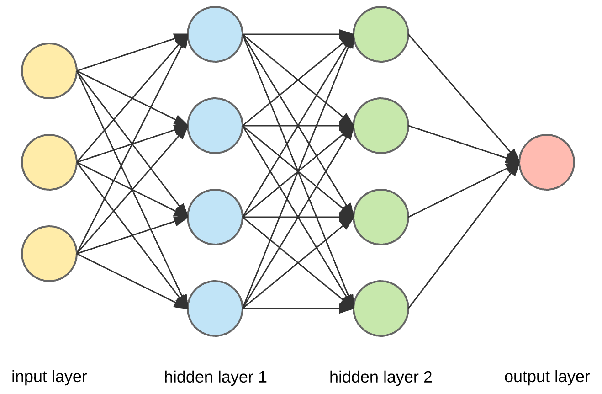
\includegraphics[width=4in]{dnn}
    % \caption[Struktura DNN - źródło: \url{https://towardsdatascience.com/building-a-convolutional-neural-network-male-vs-female-50347e2fa88b}]{Struktura DNN}
    \caption[Struktura DNN - źródło: \url{https://towardsdatascience.com}]{Struktura DNN}
    \label{fig:dnn}
  \end{figure}

  % Jedną z takich przełomowych architektur jest CNN (ang. convolutional neural
  % network). Są to sieci o hierarchicznej strukturze, gdzie obrazy wejściowe w
  % postaci macierzy wpier poddawane są ekstrakcji cech poprzez dokonanie operacji
  % konwolucji na obrazie poprzez przesuwanie zestawu filtrów wzdłuż obrazu.
  % Filtry te są zazywczaj inicjowane losowymi wartościami i w miarę trenowania,
  % dopasowują swoje parametry do wybranej problematyki.
  % Na wyjściu filtrów otrzymuje się macierze o mniejszej rozdzielczości
  % reprezentujące wyniki operacji konwolucji w danym punkcie. Otrzymane macierze
  % wyjściowe mogą być podawane na kolejne warstwy konwolucyjne w celu ekstrakcji
  % kolejnych cech. Dzięki temu procesowi kolejne warstwy filtrów uczą się
  % rozpoznawać kluczowe cechy na obrazie, od drobnych elemtów takich jak
  % krawędzie albo kształty po bardziej złożone takie jak części ciała albo
  % przedmioty.
  % Końcowe warstwy dokonują spłaszczania, czyli zamieniania wielowymiarowych
  % macierzy cech na jednowymiarowe wektore, które podawane są na wejście
  % FCL (ang. fully connected layer).

  % Lata rozwoju sztucznych sieci neuronowych zaowocowały powstaniem wielu technik służących do analizy i edycji obrazów. W poniższym rozdziale zaprezentowane zostaną, oraz pokrótce opisane, najważniejsze i najciekawsze przykłady, z których część znajdzie rozwinięcie w dalszej części tej pracy.

  \subsection{Sieci splotowe}
    \label{sieci_splotowe}

    Neuronowe sieci splotowe (CNN ang. convolutional neural network) stanowią podstawową strukturę w zakresie przetwarzania i analizowania obrazów cyfrowych. Są to sieci o hierarchicznej strukturze stanowiące podwaliny większości klasyfikatorów, detektorów, czy sieci segmentujących.

    Autorzy jednego z artykułów traktujących o sieciach splotowych \cite{cnn} opisują je następująco:
    \begin{quote}
      'CNN to skuteczny algorytm poznawczy, stosowany powszechnie przy rozpoznawaniu wzorców i przetwarzaniu obrazów. Posiada wiele cech, takich jak prosta struktura, mniej parametrów treningowych, czy zdolność do adaptacji. CNN stały się gorącym tematem w zakresie analizy głosu i rozpoznawania obrazu. Ich struktura oparta na podziale wag czyni je bardziej podobnymi do biologicznych sieci neuronowych. Redukuje to złożoność modelu sieci oraz liczbę wag'.
    \end{quote}

    Na CNN składają się zazwyczaj trzy rodzaje warstw, z których każda posiada inne cechy.

    Podstawową warstwę stanowi warstwa splotowa. Składa się ona ze zbioru filtrów (neuronów) odpowiedzialnych za ekstrakcję cech z analizowanych obrazów poprzez dokonanie operacji
    konwolucji na obrazie poprzez przesuwanie zestawu filtrów wzdłuż niego.
    Na wyjściu filtrów otrzymuje się macierze o mniejszej rozdzielczości
    reprezentujące wyniki operacji konwolucji w danym punkcie. Każda kolejna warstwa splotowa wydobywa z obrazu cechy o wyższych poziomach abstrakcji
    bazując na wynikach obliczeń poprzednich warstw tego rodzaju. Dzięki temu
    procesowi kolejne warstwy filtrów uczą się
    rozpoznawać kluczowe cechy na obrazie, od drobnych elementów takich jak
    krawędzie albo kształty po bardziej złożone takie jak części ciała albo
    całe obiekty. Filtry te są zazwyczaj inicjowane losowymi wartościami i w miarę trenowania, dopasowują swoje parametry do wybranej problematyki.

    Drugim istotnym elementem sieci splotowych jest warstwa poolingu. Może zostać opisana następująco \cite{deeplearn}:
    \begin{quote}
      'We wszystkich przypadkach pooling pomaga uczynić reprezentację w przybliżeniu niezmienną w stosunku do małych tłumaczeń danych wejściowych. Niezmienność wobec tłumaczenia oznacza, że jeśli poddamy dane wejściowe nieznacznej translacji, to wartość większości wyników poddanych poolingowi nie ulegnie zmianie'.
    \end{quote}

    Końcowy element CNN w większości przypadków stanowią warstwy gęste (FCL ang. Fully Connected Layer). Odpowiadają one za dokonanie odpowiedniej klasyfikacji obrazu na podstawie danych dostarczonych przez warstwy poprzedzające. Są przez to nieodzowne w przypadku zadań związanych z wszelkiego rodzaju klasyfikacją obrazów.

    Wymienione tutaj elementy składowe sieci splotowych mogą przyjmować różne rozmiary i występować w różnych konfiguracjach, co przedstawiono na poniższym Rysunku \ref{fig:cnn_structure}.
    \begin{figure}[h]
     \centering
     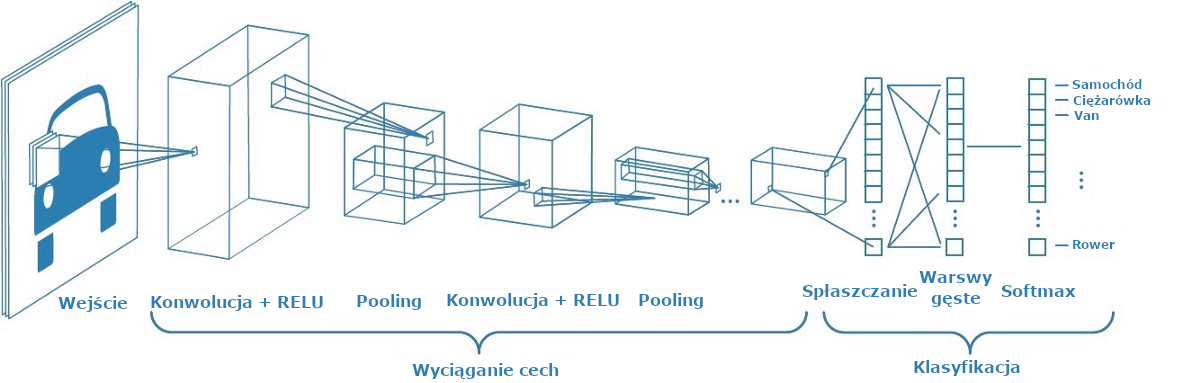
\includegraphics[width=4in]{cnn_structure}
     % \caption[Przykładowa struktura CNN - źródło: \url{https://www.mathworks.com/solutions/deep-learning/convolutional-neural-network.html}]{Przykładowa struktura CNN}
     \caption[Przykładowa struktura CNN - źródło: \url{https://www.mathworks.com}]{Przykładowa struktura CNN}
     \label{fig:cnn_structure}
    \end{figure}
    \newline
    Zapewnia to szerokie pole do eksperymentów i sprawia, że sieci te zdolne są rozwiązywać złożone, różnorodne problemy z wielu dziedzin codziennego życia.

  \subsection{FCN}

   Jednym z kluczowych problemów, jakie stawia przed badaczami edycja obrazów jest zagadnienie segmentacji semantycznej. Klasyczna klasyfikacja, polegająca na przypisywaniu obrazów do odpowiednich grup tematycznych, jest w tym przypadku sprowadzana do poziomu pojedynczych pikseli. Oznacza to, że sieci neuronowe przeznaczone do tego zadania są w stanie dokonać klasyfikacji dla każdego pojedynczego piksela analizowanego obrazu. Na tej podstawie uzyskiwany jest podział na segmenty, z których każdy reprezentuje inną klasę obiektów, jak na poniższym Rysunku \ref{fig:segmentation}.

   \begin{figure}[h]
    \centering
    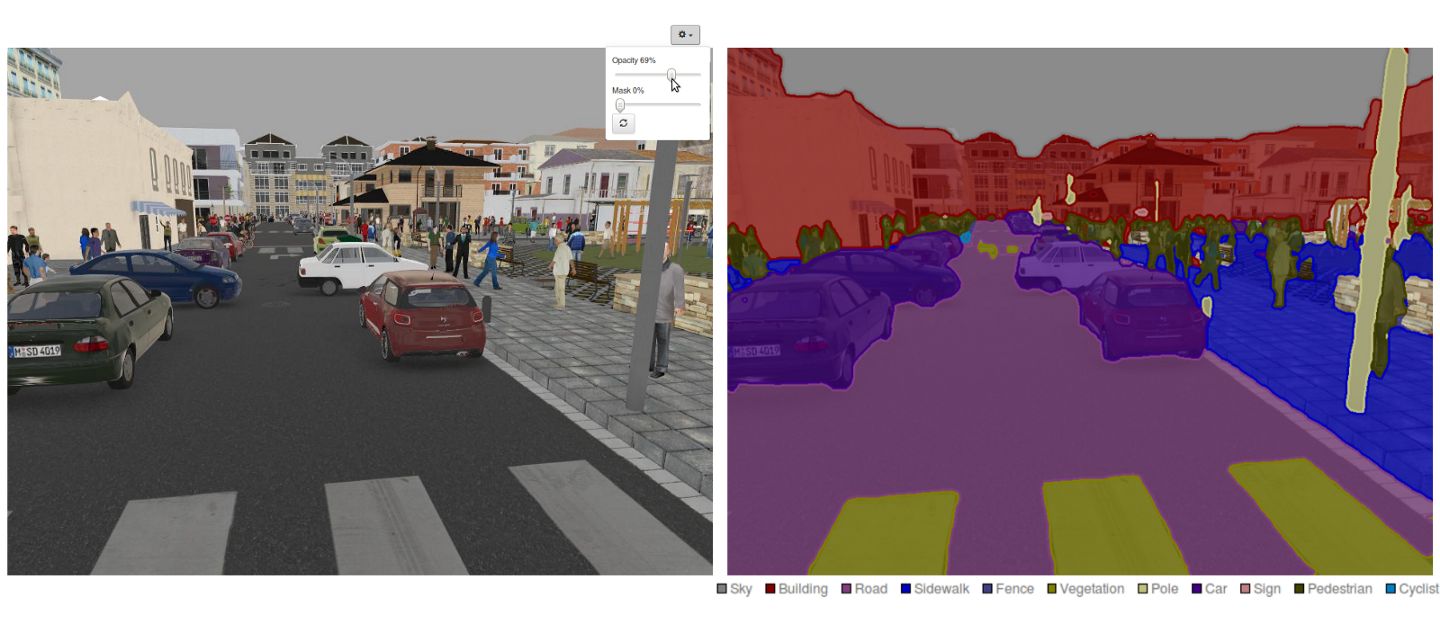
\includegraphics[width=4in]{segmentation}
    % \caption[Segmentacja semantyczna - źródło: \url{https://devblogs.nvidia.com/image-segmentation-using-digits-5/}]{Segmentacja semantyczna}
    \caption[Segmentacja semantyczna - źródło: \url{https://devblogs.nvidia.com}]{Segmentacja semantyczna}
    \label{fig:segmentation}
  \end{figure}

   W większości modele odpowiadające za przeprowadzanie segmentacji składają się z szeregowego połączenia enkodera oraz dekodera. Enkoder jest zazwyczaj pre-trenowaną siecią neuronową przeznaczoną do klasyfikowania obrazów. Dekoder odpowiada za semantyczne rzutowanie cech w niskiej rozdzielczości, wyuczonych przez enkoder, na wysoką rozdzielczość samych pikseli tworząc wspomniany wcześniej podział segmentowy.

   FCN (ang. Fully Convolutional Networks) stanowią szczególny rodzaj sieci neuronowych przeznaczonych do segmentacji obrazów. Składają się one wyłącznie z kombinacji warstw splotowych oraz poolingu. Są w stanie przetwarzać obrazy o dowolnej, zmiennej wielkości, w odróżnieniu od innych typów modeli, w których zastosowanie warstw gęstych (FCL) wymusza z góry ustalone rozmiary danych wejściowych.

   Naprzemienne przepuszczanie obrazów przez wspomniane warstwy splotowe oraz pooling może powodować niską rozdzielczość wyjściowych rezultatów pracy tych sieci oraz rozmycie granic poszczególnych obiektów. Z tego powodu w nowoczesnych rozwiązaniach stosuje się dodatkowe mechanizmy zapobiegające tego typu trendom.

  \subsection{Modele generatywne}
  \label{modele_generatywne}
   Koncepcja modeli generatywnych, w skrócie GANów, przedstawiona została w 2014 roku przez Iana Goodfellow oraz jego współpracowników na uniwersytecie w Montrealu \cite{gan}. Modele te stanowią połączenie dwóch głębokich sieci neuronowych działających przeciwstawnie do siebie nawzajem.

   Pierwsza sieć to tak zwany generator. W odniesieniu do tematu pracy, jego działanie polega na generowaniu nowych obrazów, lub ich fragmentów na podstawie wektora szumów.

   Obrazy te przekazywane są, równolegle z zestawem obrazów prawdziwych, do dyskryminatora stanowiącego drugą część modelu GAN. Działanie tej sieci neuronowej polega na określeniu (w skali 0 do 1), w jakim stopniu produkty wyjściowe generatora odpowiadają obrazom rzeczywistym.

   W opisanym modelu występuje zatem podwójna pętla sprzężenia zwrotnego. Dyskryminator określa autentyczność obrazów porównując je ze zdefiniowaną odgórnie bazą danych. Z kolei generator otrzymuje informację o skuteczności swojego działania ze strony dyskryminatora.

   Model generatywny znajduje się w stanie ciągłego konfliktu. Generator dąży do jak najdokładniejszego fałszowania obrazów w celu oszukania dyskryminatora, którego celem jest z kolei jak najdokładniejsze wykrywanie podróbek. Obie sieci neuronowe nieustannie dążą do osiągnięcia przewagi nad rywalem w procesie treningu. Ciągła rywalizacja sprawia, że zarówno generator, jak i dyskryminator zyskują coraz wyższą skuteczność działania.

   W praktyce modele generatywne są w stanie naśladować dowolną dystrybucję danych. Są w stanie kreować światy podobne do naszego w zakresie obrazu, dźwięku czy mowy. Można powiedzieć, że są to prawdziwi syntetyczni artyści.


\section[Przegląd rozwiązań (Bartosz Bieliński)]{Przegląd rozwiązań}

  Na przestrzeni ostatnich paru lat pojawiło się wiele innowacyjnych technologii opartych
  na sieciach neuronowych. Takie cechy sieci, jak niezwykłe zdolności do generalizacji
  zdobytej wiedzy na nowe przypadki oraz olbrzymia elastyczność sprawiły, że
  znalazły one wiele rzeczywistych zastosowań, zwłaszcza do problemów
  nieszablonowych, dla których metody nie oparte na uczeniu maszynowym
  nie przynosiły zadowalających wyników. Zastosowania te często były
  przełomowe w swojej dziedzinie i do czasów dzisiejszych uważane są
  za prekursorów pewnych idei.

  W tym rozdziale skupiono się na przedstawieniu kilku interesujących rozwiązań
  stosujących sieci neuronowe do edycji obrazu, które są zarazem kluczowe do lepszego
  zapoznania się z omawianą problematyką.

  \subsection{Colorful image colorization}

    Wraz z rozwojem sieci neuronowych, rosło zainteresowanie możliwościami zastosowania
    ich do kolorowania czarno-białych obrazów. Jedno z dostępnych rozwiązań tego
    zagadnienia zostało przedstawione przez grupę pracowników Uniwersytetu w
    Berkeley \cite{colorful_image_colorization}. Celem ich pracy było stworzenie
    modelu, który niekoniecznie odtwarza oryginalne barwy obrazu, ale generuje
    barwy prawdopodobne, zdolne przekonać ludzkiego obserwatora o autentyczności
    obrazu. Uzyskane rezultaty zostały przedstawione na
    Rysunku \ref{fig:colorful_image_colorization}.

    \begin{figure}[ht]
      \centering
      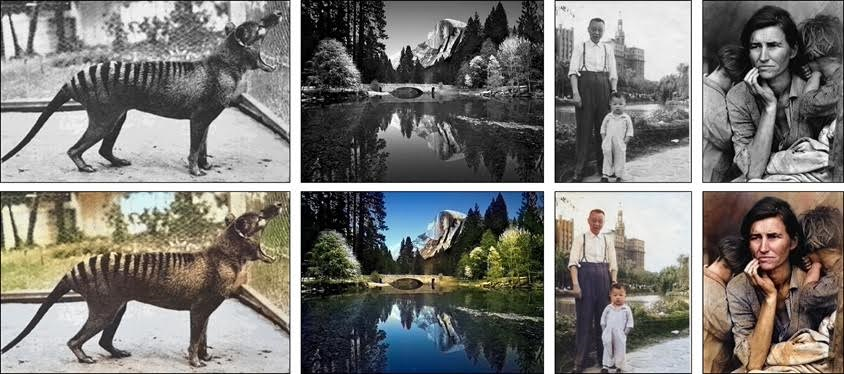
\includegraphics[width=4in]{image_colorization}
      \caption[Efekt kolorowanie czarno-białych obrazów przez wytrenowany model - źródło:
      \cite{colorful_image_colorization}]{Efekt kolorowanie czarno-białych obrazów przez wytrenowany model.}
      \label{fig:colorful_image_colorization}
    \end{figure}

    Wykorzystany model składa się z wielu warstw CNN, w których skład wchodzą
    warstwa filtrów konwolucyjnych, warstwa ReLU (ang. Rectified
    Linear Unit) oraz warstwa BatchNorm (ang. Batch normalization).
    Aby zapobiec utracie informacji przestrzennych, sieć nie posiada warstw poolingu.
    Istotny był także sposób
    przygotowania zbioru danych do trenowania modelu. Obrazy ze zbioru uczącego
    były wpierw konwertowane do modelu barw YUV. Kanał Y był podawany na
    wejście sieci, a kanały UV pełniły funkcję pożądanej odpowiedzi w uczeniu
    nadzorowanym.

    Ważnym aspektem zbadanym w artykule było także dobranie odpowiedniej
    funkcji kosztu. Nieodpowiedni wybór skutkował desaturacją kolorowanych
    obrazów. Jedną z potencjalnych przyczyn tego zjawiska może być tendencja
    sieci do tworzenia bardziej konserwatywnych odpowiedzi. Aby zniwelować ten
    efekt, w modelu została zastosowana specjalna technika modyfikacji
    funkcji kosztu. Polega ona na przewidywaniu dystrybucji możliwych kolorów
    dla każdego piksela i poprawie wartości wyliczanego dla modelu błędu, w celu
    wyróżnienia rzadko spotykanych kolorów.

    Powstałe rozwiązanie dowodzi olbrzymiego potencjału zastosowania sieci
    neuronowych w dziedzinie pracy nad obrazami, efekty uzyskiwane za ich pomocą
    są niemożliwe do odtworzenia z użyciem tradycyjnych algorytmów.

  \subsection{Image Style Transfer Using Convolutional Neural Networks}

    W roku 2016 został przedstawiony światu \textit{A Neural Algorithm of Artistic Style}
    \cite{image_style_transfer}. Wprowadzał on przełom w dziedzinie przenoszenia
    stylu jednego obrazu na inny, a jego sukces opierał się na właściwym wykorzystaniu
    konwolucyjnych sieci neuronowych. Podstawą tego osiągnięcia było odkrycie przez
    Leona A. Gatys oraz jego współpracowników, że w CNN reprezentacja treści
    obrazu oraz jego stylu jest rozłączna. Umożliwia to wydobycie stylu
    przetwarzanego obrazu oraz połączenie go z treścią innego obrazu, czego
    dokonuje właśnie \textit{A Neural Algorithm of Artistic Style}. Rezultaty takich
    operacji można zaobserwować na Rysunku \ref{fig:image_style_transfer}

    \begin{figure}[H]
      \centering
      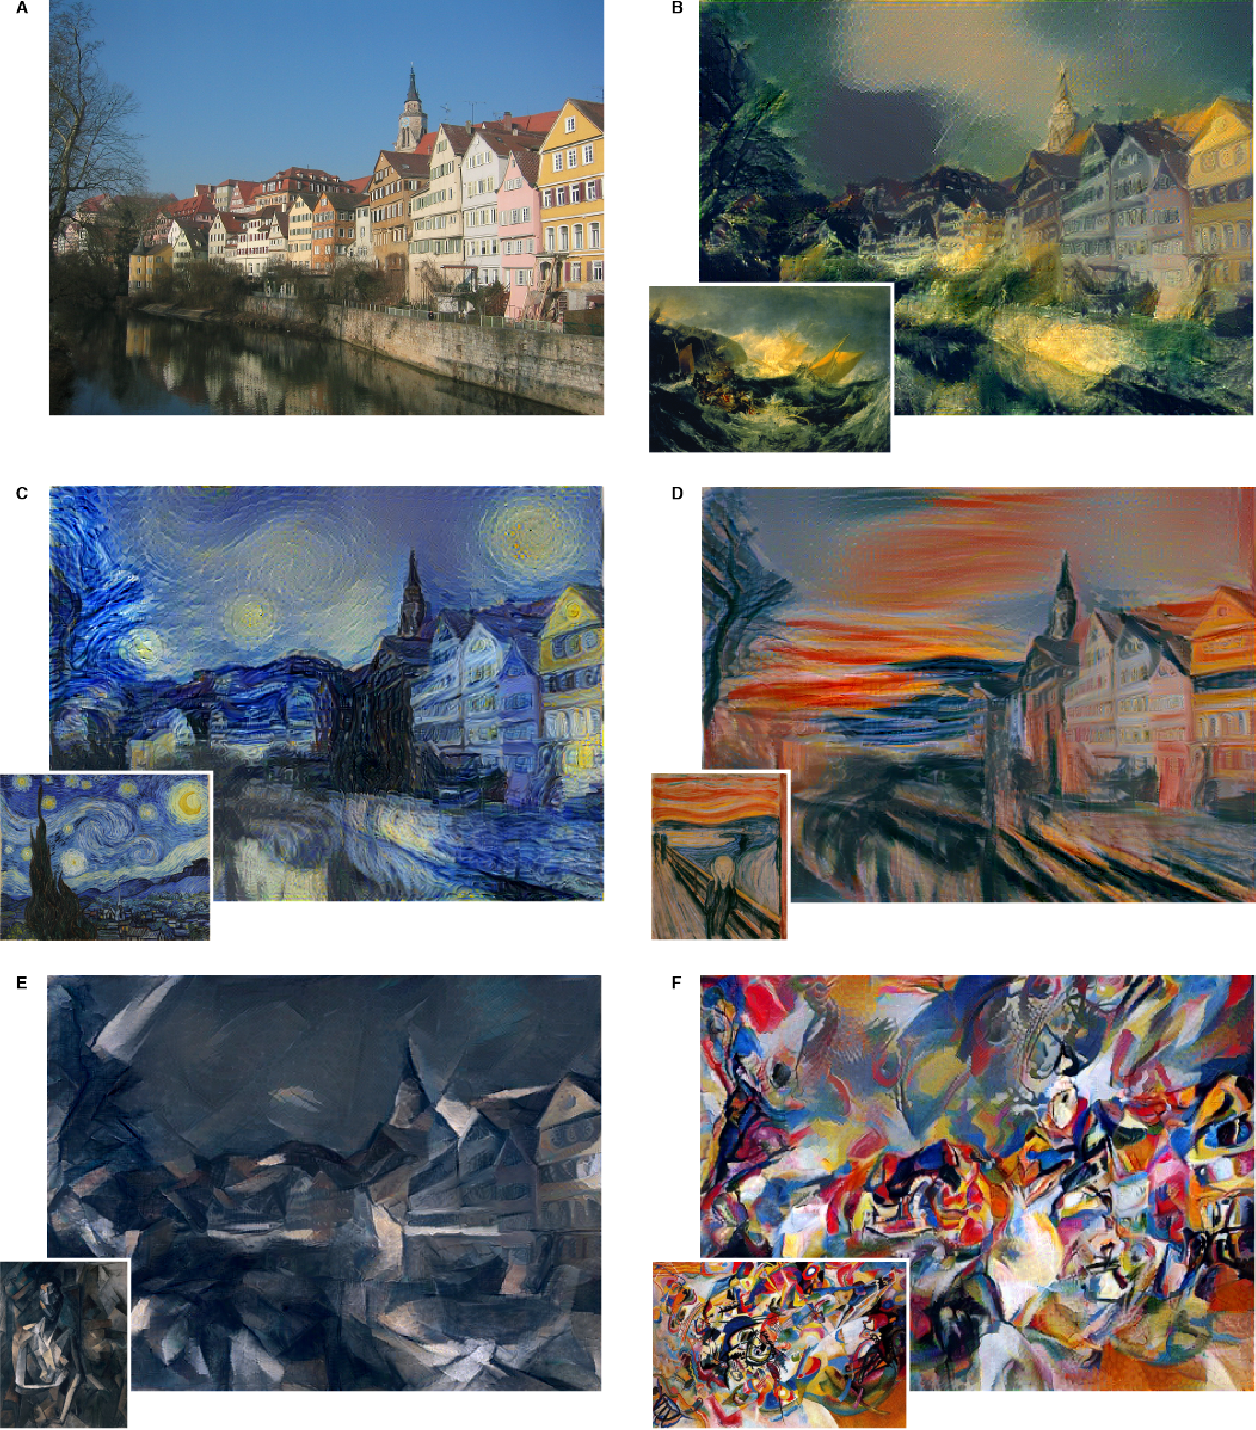
\includegraphics[width=4in]{image_style_transfer}
      \caption[Obrazy będące kombinacją treści zdjęcia ze stylami kilku znanych dzieł sztuki - źródło:
      \cite{image_style_transfer}]
      {Obrazy będące kombinacją treści zdjęcia ze stylami kilku znanych dzieł sztuki.}
      \label{fig:image_style_transfer}
    \end{figure}

    Do zbudowania modelu zostały użyte warstwy konwolucyjne oraz poolingu z
    architektury VGG-Network \cite{vgg_network}, która została wytrenowana pod
    kątem rozpoznawania obiektów i określania ich położenia. Dzięki temu sieć
    przetwarzając obraz tworzy jego reprezentację, która wraz z
    kolejnymi warstwami, przedstawia coraz pełniejszą informację o obiektach,
    a niekoniecznie o dokładnym wyglądzie obrazu.
    W modelu nie została użyta ani jedna warstwa gęsta, dzięki czemu na wyjściu
    możliwe jest otrzymanie dwuwymiarowego obrazu.
    Dla lepszej syntezy obrazów, w warstwach
    łączących zastosowano próbkowanie wartością średnią, zamiast najczęściej
    stosowaną wartością maksymalną.
    Takie zabiegi umożliwiają wyliczenie reprezentacji stylu z korelacji
    pomiędzy poszczególnymi cechami w kolejnych warstwach konwolucyjnych.

    Cały proces renderowania polega na odpowiednim przechowaniu w modelu treści
    oraz stylu wejściowych obrazów i składa się z wielu następujących po sobie etapów.
    Wpierw obraz, z którego pobierany jest styl, jest podawany na
    wejście sieci oraz przetwarzany, reprezentacja stylu, wyselekcjonowana z
    właściwych warstw, jest odpowiednio przechowywana. Następnie temu samemu
    procesowi poddawany jest obraz z treścią, ale reprezentacja treści jest wyciągana z ostatnich
    warstw konwolucyjnych.
    W celu wykonania fuzji obrazów, uzyskane reprezentacje treści oraz stylu są
    zapisywane w tych warstwach modelu skąd zostały odczytane, po czym na wejście
    podawany jest obraz składający się z losowego szumu białego.
    Następnie, poprzez iteracyjną minimalizację funkcji kosztu, obraz wejściowy jest modyfikowany, co w rezultacie końcowym doprowadza do nałożenia zapisanego
    stylu na wczytaną treść.

    \textit{A Neural Algorithm of Artistic Style} jest świetnym przykładem, jak elastyczne
    mogą być interfejsy do modyfikacji obrazu oparte na technologii sieci neuronowych.

  \subsection{Invertible Conditional GANs for image editing}
    Edycja obrazów może być dokonywana na wielu różnych poziomach zaawansowania
    i abstrakcji, operacje niezłożone, takie jak nakładanie filtrów, mogą być
    wykonywane przez proste algorytmy. Jednak w przypadku próby modyfikacji
    elementów na obrazie, algorytmy te nie będą w stanie dokonać semantycznych
    zmian, ze względu na brak możliwości zrozumienia treści obrazu. Rozwiązanie
    tego problemu zostało przedstawione w postaci modelu IcGAN
    (ang. Invertible conditional Generative Adversarial Network) w roku 2016
    \cite{gan_editing}. Zaprezentowany model to enkoder z możliwością
    generowania wektora informacji o atrybutach obrazu, połączony z warunkowym
    GANem zdolnym do kontrolowania cech generowanych obrazów na podstawie dodatkowej
    informacji warunkowej. Takie działanie umożliwia wprowadzanie zmian w
    atrybutach generowanego obrazu uzyskiwanego na wyjściu cGAN (ang. conditional Generative
    Adversarial Network). Rezultaty działania modelu można zaobserwować na
    Rysunku \ref{fig:IcGAN}

    \begin{figure}[ht]
      \centering
      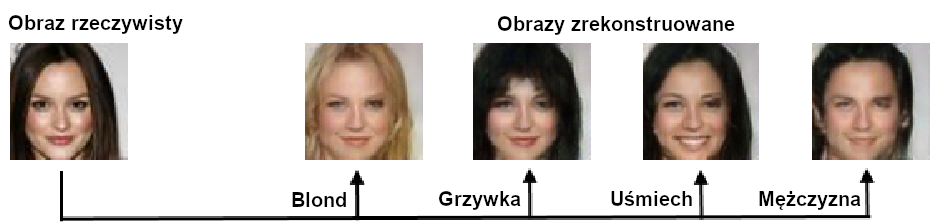
\includegraphics[width=4in]{IcGAN}
      \caption[Obrazy generowane przez IcGAN - źródło: \cite{gan_editing}]{Obrazy generowane przez IcGAN.}
      \label{fig:IcGAN}
    \end{figure}

    Wykorzystany w IcGAN ekonder w rzeczywistości składa się z dwóch podrzędnych
    enkoderów. Enkoder $E_{z}$ koduje wejściowy obraz do utajonego wektora $z$ reprezentacji
    obrazu, natomiast enkoder $E_{y}$ generuje wektor informacji $y$, oddający
    pewne kluczowe atrybuty obrazu. Enkodery są trenowane z użyciem już wytrenowanego
    cGAN oraz obrazów rzeczywistych z etykietami ze zbioru uczącego. Zbadane
    zostały także różne podejścia interakcji między dwoma enkoderami, wyróżnić
    można podejście, w którym enkodery są w pełni niezależne, podejście
    gdzie wyjście $E_{z}$ jest zależne od wyjścia $E_{y}$, a także podejście
    gdzie $E_{z}$ oraz $E_{y}$ są połączone w jeden enkoder o współdzielonych
    warstwach i dwóch wyjściach.

    W przypadku cGAN można wyróżnić dwa najważniejsze czynniki, które trzeba
    mieć na uwadze. Pierwszym jest źródło wektora $y$ podawanego na
    generator. W przypadku dyskryminatora, $y$ jest pobierany ze
    zbioru treningowego, jednakże w przypadku podawania tego
    samego wektora na generator, pojawia się możliwość wystąpienia niepożądanego
    przeuczenia modelu. Autorzy artykułu dokonali analizy tego rozwiązania,
    a także zbadali wydajność metod Bezpośredniej Interpolacji oraz
    Jądrowego Estymatora Gęstości. Wynikiem tych badań było stwierdzenie, że
    dla danej problematyki najlepiej sprawdza się podawanie wektora $y$ ze zbioru
    uczącego. Możliwość przeuczenia modelu została skomentowana następująco:
    \begin{quote}
      % This is only likely to occur if the conditional information
      % is, to some extent, unique for each image. In the case where the attributes of an image are binary, one attribute vector y could describe a varied and large enough subset of images, preventing the model from overfitting given y.
      'Jest to możliwe tylko, gdy informacje warunkowe są do pewnego stopnia
      unikatowa dla każdego obrazu. W tym przypadku, gdzie atrybuty obrazów są
      binarne, jeden wektor $y$ może opisać wystarczająco duży i zróżnicowany
      podzbiór obrazów, zapobiegając nadmiernemu dopasowaniu się modelu do
      danego $y$.'
    \end{quote}

    Drugim czynnikiem jest warstwa generatora i dyskryminatora cGAN na
    którą podany jest wektor $y$. Guim Perarnau oraz jego współpracownicy ustalili, że najlepsze rezultaty otrzymuje się po podaniu wektora $y$ na warstwę wejściową
    generatora oraz pierwszą warstwę konwolucyjną dyskryminatora.

    Ważnym spostrzeżeniem z analizy rozwiązania IcGAN jest obecność
    olbrzymiej liczby różnorodnych rozwiązań opartych na sieciach neuronowych.
    Coraz to nowe architektury zostają wynalezione, aby udoskonalić
    zastosowania sieci neuronowych do przetwarzania i modyfikowania obrazów.

  \subsection{Neural photo editing}
    W 2017 roku Andrew Brock, Theodore Lim, J.M. Ritchie and Nick Weston
    zaprezentowali \textit{Neural Photo Editor} \cite{neural_photo_editor}, narzędzie
    do edytowania obrazu wyposażone w mechanizmy wykrywania kontekstu zmiany.
    Twórcy opisują swoje dzieło następująco:

    \begin{quote}
      % 'An interface that leverages the power of generative neural networks to
      % make large, semantically coherent changes to existing images.'
      'Interfejs wykorzystujący moc generatywnych sieci neuronowych do
      wprowadzania dużych, semantycznie spójnych zmian w istniejących obrazach.'
    \end{quote}

    Użytkowanie wygląda następująco: użytkownik pędzlem o określonym kolorze i
    rozmiarze maluje na wybranym obrazie, jednak zamiast zmieniać wartości
    pojedynczych pikseli, interfejs odczytuje kontekst wprowadzanej edycji.
    Następnie na jego podstawie wprowadza zmiany
    semantyczne w kontekście żądanej zmiany koloru. Efekt działania interfejsu
    został przedstawiony na Rysunku \ref{fig:npe}.

    \begin{figure}[ht]
      \centering
      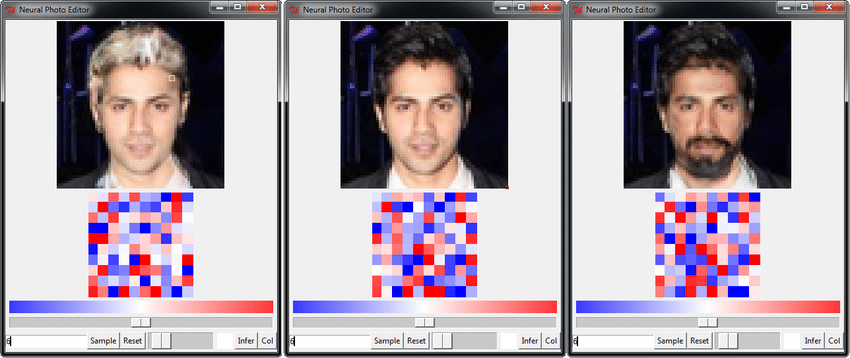
\includegraphics[width=4in]{NPE}
      \caption[Efekt działania \textit{Neural Photo Editor} - źródło: \cite{neural_photo_editor}]
      {Efekt działania Neural Photo Editor.}
      \label{fig:npe}
    \end{figure}

    Skuteczność NPE (ang. Neural Photo Editor) polega na zastosowaniu IAN
    (ang. Introspective Adversarial Network), czyli sieci złożonej z połączonych
    VAE (ang. Variational Autoencoder) \cite{vae} oraz GANów, w taki sposób, że dekodująca
    sieć autoenkodera jest używana jako sieć generująca w GANie.
    Poprzez przechwytywanie przez model dalekosiężnych zależności, wykorzystanie
    bloku obliczeniowego bazującego na rozszerzonych splotach o
    współdzielonych wagach oraz dzięki zastosowaniu ulepszonej generalizacji,
    udało się osiągnąć dokładną rekonstrukcję obrazu bez strat na jakości detali.

    Powstanie NPE utwierdza w przekonaniu, że aktualnie istniejące sieci
    neuronowe do edycji obrazu znacznie przewyższają zwykłe algorytmy pod
    względem możliwości, a także są zauważalnie słabiej uzależnienie od wkładu
    ludzkiego.


\section{Przebieg projektowania sieci neuronowych}

\section{Podsumowanie}


\newpage
\begin{thebibliography}{99} %{99} numery co najwyżej dwucyfrowe
  \bibitem{gan} Ian J.~Goodfellow, Jean~Pouget-Abadie, Mehdi~Mirza, Bing~Xu, David~Warde-Farley, Sherjil~Ozair, Aaron~Courville, Yoshua~Bengio:
    \emph{Generative Adversarial Networks}, ('2014)

    \bibitem{neural_photo_editor} Andrew Brock, Theodore Lim, J.M. Ritchie,
    Nick Weston:
      \emph{NEURAL PHOTO EDITING WITH INTROSPECTIVE ADVERSARIAL NETWORKS}, ('2017)

\end{thebibliography}

\section*{Załączniki}
\addcontentsline{toc}{section}{Załączniki}  % Dodanie to TOC
  \tab Załączniki i dodatki\:



\end{document}
